\subsection{Multiple Testing}
Given nulls $H_{0,1}, \dots, H_{0,m}$ with p-values $p_1,\dots, p_m$. The goal is to identify \underline{subset of nulls} for which we are confident that the null is false. 

\begin{defn}[Multiple Testing]
    Multiple testing procedure is a map $(p_1,\dots,p_m) \mapsto$ subset of $\{1,\dots,m\}$ (the discoveries).
\end{defn}
\emph{\textbf{Note.}} This may also include side information / co-variates / clustering of hypotheses.

Possible goals/measures of error:
\begin{itemize}
    \item Family-wise Error Rate (FWER): $\mathbb{P}\{\textup{Any false discoveries}\}$
    \item False Discovery Rate (FDR): $\mathbb{E}\left[\frac{\textup{\# false discoveries}}{\textup{\# discoveries}}\right]$
    \item False Discovery Exceeds (FDX): $\mathbb{P}\left\{\textup{FDP} \geq \alpha \right\}$
\end{itemize}

\begin{proposition}[Holm-Bonferroni]
Run Bonferroni on $p_1,\dots,p_m$. Label smallest $p_i$ as discovery, remove it and rerun until we stop rejecting the global null.
\end{proposition}

Let $p_{(1)}\leq \cdots \leq p_{(n)}$ be sorted p-values, then the discoveries by Holm-Bonferroni are given by $\{p_{(1)}, \dots, p_{(m)} \}$, where $\hat{k} := \min\{k \in \{1,\dots,m\} \colon p_{(k)} > \frac{\alpha}{m+1-k}\}$. If $\hat{k} = 1$, then discoveries is $\emptyset$.

\emph{\textbf{Note.}} This procedure is more powerful than the Bonferroni procedure, which rejects any $p_i \leq \frac{\alpha}{m}$.

\begin{thm}{Holm-Bonferroni FWER}{HB FWER}
 Holm-Bonferroni satisfies FWER $\leq \alpha$.
\end{thm}

\begin{pr}
    Let $m_0$ be the number of true nulls. First, note
    \begin{align*}
        \mathbb{P}\left\{p_i \leq \frac{\alpha}{m_0} \textup{ for any true }H_{0,i} \right\} \leq \alpha.
    \end{align*}

    We claim that if we make more than 1 false discovery, then $p_i \leq \frac{\alpha}{m_0}$ holds  for some true $H_{0,i}$, which in turn implies 
    $$\textup{FWER} \leq  \mathbb{P}\left\{p_i \leq \frac{\alpha}{m_0} \textup{ for any true }H_{0,i} \right\} \leq \alpha.$$

    Let $k$ be the smallest value such that $p_{(k)}$ corresponds to a true null. Then, $\textup{FWER} = \mathbb{P}[\hat{k}>k]$. If $\hat{k} > k$, Holm-Bonferroni rejects $p_{(k)}$ and $p_{(k)} \leq \frac{\alpha}{m+1-k} \leq \frac{\alpha}{m_0}$ holds true.
\end{pr}

\begin{proposition}[Benjamini-Hochberg]
    Benjamini-Hochberg (BH) rejects $p_{(1)}, \dots p_{(\hat{k})}$ where $\hat{k} = \max\{k\in\{1,\dots,m\}\colon p_k \leq \frac{\alpha k}{m}\}$.
\end{proposition}

\emph{\textbf{Step-up and Step-down:}} Given thresholds $\alpha_1 \leq \cdots \leq \alpha_m$. For Holm-Bonferroni $\alpha_k = \frac{\alpha}{m+1-k}$ and for Benjamini-Hochberg $\alpha_k = \frac{\alpha k}{m}$. Compare $p_{(k)}$ against $\alpha_k$.
\begin{itemize}
    \item Step-down: reject $p_{(1)}, \dots, p_{(\hat{k}-1)}$, where $\hat{k} = \min\{k \in \{1,\dots,m\}\colon p_{(k)} > \alpha_k\}$
    \item Step-up: reject $p_{(1)}, \dots, p_{(\hat{k}-1)}$, where $\hat{k} = \max\{k \in \{1,\dots,m\}\colon p_{(k)} \leq \alpha_k\}$
\end{itemize}

\textbf{\underline{Intuition behind BH}}\\
Suppose we reject all $p_i \leq t$
\begin{align*}
    \textup{FDP}(t) = \frac{\textup{\# true nulls with } p_i\leq t}{\textup{total \# hypotheses with } p_i\leq t}
\end{align*}
We can estimate the numerator as $m\cdot t$, where $m$ is an upper bound on the number of true nulls and $t$ is an upper bound on $\mathbb{P}\{p_i\leq t\}$ for each null and $\hat{\textup{FDP}}(t) = \frac{mt}{\textup{\# }p_i\leq t}$. 

The claim is that choosing $t = \max\{k \in \{1,\dots,m\}\colon \hat{\textup{FDP}}(t) \leq \alpha \}$ and rejecting all $p_i\leq t$ is equivalent to BH. BH rejects all $i\in\{1,\dots,m\}$ with $p_i \leq \frac{\alpha \hat{k}}{m}$ and finally we have $p_{(\hat{k}+1)} > \frac{\alpha\hat{k}}{m}$. $\hat{\textup{FDP}}(t)$ at $t = \frac{\alpha\hat{k}}{m}$ is $\frac{mt}{\textup{\# }p_i\leq t} = \alpha$.

In summary,
\begin{table}[h]
\centering
\small
\renewcommand{\arraystretch}{1.2}
\begin{tabular}{ccc}
\toprule
\textbf{Testing $H_{0, \text{global}}$} & & \textbf{Multiple Testing} \\ 
\cmidrule{1-1} \cmidrule{3-3}
Bonferroni / Simes & & Bonferroni \\
\addlinespace[0.5em]
$\downarrow$ & \textit{reject iff $>1$ discovery} & $\downarrow$ \\
\addlinespace[0.5em]
Holm-Bonferroni (FWER) & & Benjamini-Hochberg (FDR) \\ 
\bottomrule
\end{tabular}
\end{table}

\datum{Lecture 4: 01/15}
\emph{\textbf{Question:}} When do we expect BH to work well, i.e. FDR $\leq \alpha$ while making as many discoveries as possible.

\emph{\textbf{Even stronger goal:}} Want FDP $\lesssim \alpha$ with high probability.
\begin{itemize}
    \item True, as long as $p_i$ are independent or weakly independent and rejection threshold not too close to 0, i.e. \# rejections not too small
\end{itemize}

\begin{figure}[h!]
    \centering
\begin{tikzpicture}[scale=0.6]
\begin{axis}[
    width=11cm,
    height=7cm,
    xlabel={P-value},
    ylabel={Density},
    xmin=0, xmax=1,
    ymin=0, ymax=4,
    xtick={0, 0.2, 0.4, 0.6, 0.8, 1},
    xticklabels={0, $t$, 0.4, 0.6, 0.8, 1},
    ytick={1},
    yticklabels={1},
    axis lines=left,
    enlarge x limits=false,
    legend style={at={(0.5,-0.2)}, anchor=north, legend columns=-1, draw=none}
]

% 1. Denominator R(t): Only shade bars <= t
% Signal Region (0 to t)
\addplot+[
    ybar interval,
    fill=blue!25,
    draw=blue!40!black,
    area legend
] coordinates {
    (0, 3.8) (0.05, 3.4) (0.10, 2.8) (0.15, 2.0) (0.20, 0)
};
\addlegendentry{Denominator \quad}

% 2. Non-Discoveries: Outlined only (not part of the formula)
\addplot+[
    ybar interval,
    fill=none,
    draw=gray!50,
    forget plot
] coordinates {
    (0.20, 1.2) (0.25, 0.9) (0.30, 0.85) (0.35, 0.8) 
    (0.40, 0.82) (0.45, 0.78) (0.50, 0.81) (0.55, 0.79) 
    (0.60, 0.8) (0.65, 0.82) (0.70, 0.77) (0.75, 0.81) 
    (0.80, 0.8) (0.85, 0.79) (0.90, 0.82) (0.95, 0.8) (1, 0)
};

% 3. Numerator: m * t (Expected False Discoveries)
\addplot[
    fill=red, 
    fill opacity=0.3, 
    postaction={pattern=north east lines, pattern color=red!70},
    draw=red,
    line width=1.2pt
] coordinates {
    (0,0) (0,1) (0.20,1) (0.20,0)
} -- cycle;
\addlegendentry{Numerator}

% 4. Vertical threshold line
\draw [black, ultra thick] (axis cs:0.20,0) -- (axis cs:0.20,4);
\node at (axis cs:0.22, 3.5) [anchor=west] {Rejection Threshold $t$};

% 5. Horizontal null line
\draw [red, thick, dashed] (axis cs:0,1) -- (axis cs:1,1);

\end{axis}
\end{tikzpicture}
\caption{FDP visualized}
\end{figure}

$\hat{\textup{FDP}}(t) \approx \textup{FDP}(t)$ holds as long as the histogram of $\{p_i \colon H_{0,i} \textup{ is true} \}$ is $\approx m_0 / m \textup{ draws from Uniform}[0,1] $, where $m_0$ is number of true nulls. This may fail if null $p_i$ are not independent.

\begin{table}[h]
\centering
\begin{tabular}{|l|c|c|}
\hline
 & \textbf{FDX Control} & \textbf{FDR Control} \\ \hline
Independent $p_i$ & \begin{tabular}[c]{@{}c@{}}Yes (as long as \\ \# discoveries $\gg 0$)\end{tabular} & Yes \\ \hline
PRDS & No & Yes \\ \hline
Arb. independence & No & \begin{tabular}[c]{@{}c@{}}Yes \\ $\alpha \approx \alpha(1+1/2+\dots+1/m)$ \end{tabular} \\ \hline
\end{tabular}
\end{table}

\begin{thm}{Benjamini-Hochberg FDR Bound I}{BH FDR Bound I}
If $p_1,\dots,p_m$ are independent, then Benjamini-Hochberg satisifes FDR $\leq \alpha\frac{m_0}{m}$. If $p_1,\dots,p_m$ are uniform, it holds with equality.
\end{thm}

\begin{pr}
\begin{align*}
    \textup{FDR} &= \mathbb{E}\left[\frac{\sum_{\textup{null}_i}\mathbbm{1}(\{H_{0,\textup{i} } \textup{ rej}\})}{\hat{k}} \right] 
    = \sum_{\textup{null}_i} \mathbb{E}\left[\frac{\mathbbm{1}(\{H_{0,\textup{i} } \textup{ rej}\})}{\hat{k}} \right]
    = \sum_{\textup{null}_i} \mathbb{E}\left[\frac{\mathbbm{1}(\{p_i \leq \frac{\alpha \hat{k}}{m}\})}{\hat{k}} \right].
\end{align*}

\begin{lemma}
    Let $\hat{k}_{i\rightarrow 0}$ be the $\textup{outcome of BH when replacing } p_i$ with 0, i.e. run $p_1,\dots,0, p_{i+1}, \dots, p_m$.
    Then there are two possibilities
        \begin{enumerate}
            \item[(1)] $p_i \leq \frac{\alpha \hat{k}}{m} = \frac{\alpha\hat{k}_{i\rightarrow 0}}{m}$
            \item[(2)] $p_i > \frac{\alpha \hat{k}_{i\rightarrow 0}}{m} > \frac{\hat{k}}{m}$
        \end{enumerate}
\end{lemma}
By the lemma, if (1) holds, then $\hat{k} = \hat{k}_{i\rightarrow 0}$ and
\begin{align*}
    \frac{\mathbbm{1}(\{p_i \leq \frac{\alpha \hat{k}}{m}\})}{\hat{k}} = \frac{\mathbbm{1}(\{p_i \leq \frac{\alpha \hat{k}_{i\rightarrow 0}}{m}\})}{\hat{k}_{i\rightarrow 0}}.
\end{align*}

If (2) holds, then $\mathbbm{1}(\{p_i \leq \frac{\alpha \hat{k}}{m}\}) = \mathbbm{1}(\{p_i \leq \frac{\alpha \hat{k}_{i\rightarrow 0}}{m}\}) = 0$, so same equality holds. Substituting this back into the initial equation results in
\begin{align*}
    \textup{FDR} &= \sum_{\textup{null}_i} \mathbb{E}\left[\frac{\mathbbm{1}(\{p_i \leq \frac{\alpha \hat{k}}{m}\})}{\hat{k}} \right] \\
    &= \sum_{\textup{null}_i} \mathbb{E}\left[\frac{\mathbbm{1}(\{p_i \leq \frac{\alpha \hat{k}_{i\rightarrow 0}}{m}\})}{\hat{k}_{i\rightarrow 0}} \right] \\
    &= \sum_{\textup{null}_i} \mathbb{E}\left[ \mathbb{E}\left[\frac{\mathbbm{1}(\{p_i \leq \frac{\alpha \hat{k}_{i\rightarrow 0}}{m}\})}{\hat{k}_{i\rightarrow 0}} \, \Bigg\vert \, \hat{k}_{i\rightarrow 0} \right]\right]\\
    &\leq \sum_{\textup{null}_i}\frac{\frac{\alpha\hat{k}_{i\rightarrow 0}}{m}}{\hat{k}_{i
    \rightarrow 0}} = \alpha \frac{m_0}{m},
\end{align*}
whereby the inequality follows from the independence between $p_i$ and $\hat{k}_{i\rightarrow 0}$.
\end{pr}

\begin{pr}{\textbf{Lemma 1.3.4}}

First, note that $\hat{k}_{i\rightarrow 0} \geq \hat{k}$ holds because BH's number of discoveries can only increase if p-value decrease. So either $\hat{k} = \hat{k}_{i\rightarrow 0}$ holds and we want to show $p_i \leq \frac{\alpha \hat{k}}{m}$ or $\hat{k} < \hat{k}_{i\rightarrow 0}$ and we want to show $p_i > \frac{\alpha\hat{k}_{i\rightarrow 0}}{m}$.
\begin{itemize}
    \item If $\hat{k} = \hat{k}_{i\rightarrow 0}$, consider $k = \hat{k} + 1$. There are $\hat{k}$ many $p_i$ with $p_i \leq \frac{\alpha \hat{k}}{m} \leq \frac{\alpha k}{m}$. If $p_i > \frac{\alpha\hat{k}}{m}$, then it is not part of this set, so $p_1, \dots, p_{i-1}, 0, p_{i+1},\dots,p_m$ has $k$ many values less than $\frac{\alpha k}{m}$, which implies $\hat{k}_{i\rightarrow 0} \geq k$, which is a contradiction.

    \item If instead $\hat{k} < \hat{k}_{i\rightarrow 0}$, let $k = \hat{k}_{i\rightarrow 0}$. By definition of BH, there are strictly less than $k$ $p_i$ with $p_i \leq \frac{\alpha k}{m}$. But there $k$ values in $p_1, \dots, p_{i-1}, 0, p_{i+1},\dots,p_m$ with $p_i\leq \frac{\alpha k}{m}$. The only difference in these lists is $p_i$, which implies $p_i > \frac{\alpha k}{m}$.
\end{itemize}
\end{pr}

\begin{thm}{Benjamini-Hochberg FDR Bound II}{BH FDR Bound II}
Benjamini-Hochberg satisfies $\textup{FDR} \leq \alpha\frac{m_0}{m}\underbrace{\left(1+\frac{1}{2} + \dots + \frac{1}{m}\right)}_{\approx \log(m)}$ with no assumptions on dependence.
\end{thm}
\begin{pr}
    Similar to Simes.
\end{pr}

A comparison of the results between BH and Simes. If all nulls are true
\begin{align*}
    \textup{FDP} = \frac{\textup{\# false discoveries}}{\textup{total \# discoveries}} = \frac{\textup{total \# discoveries}}{\textup{total \# discoveries}} = \mathbbm{1}_{\left\{\geq \textup{1 discoveries}\right\}} = \mathbbm{1}_{\left\{\geq \textup{1 false discoveries}\right\}},
\end{align*}
i.e. $\mathrm{FDR}=\mathbb{E}[\mathrm{FDP}]=\mathbb{P}(\text{at least one rejection})=\mathrm{FWER}.$

\emph{\textup{Note.}} Under the global null $H_{0,\textup{global}}$, BH is equivalent to Simes theorem. 
\begin{pr}[Idea]
INSERT
\end{pr}


\begin{thm}{Benjamini-Hochberg FDR Bound III}{BH FDR Bound III}
If p-values satisfy PRDS, then Benjamini-Hochberg satisfies $\textup{FDR} \leq \alpha\frac{m_0}{m}$.
\end{thm}

\emph{\textbf{Note.}} This provides the same guarantee as independence of p-values and specializes to Simes result if $H_{0,\textup{global}}$ is true. However, FDP may be highly variable.

\begin{example}
    $p_i \sim U[0,1]$ and $p_1=\dots=p_m$ with probability $\alpha$
    \begin{align*}
        \begin{cases}
            p_1 \leq \alpha & \textup{reject all } H_{0,i} \textup{ and FDP = 1}, \\
            p_1 > \alpha & \textup{no discoveries } \textup{ and FDP = 0}.
        \end{cases}
    \end{align*}
\end{example}


\datum{Lecture 5: 01/20}
Define $\pi_0 := \frac{m_0}{m}$, then choosing the significance level at $\frac{\alpha}{\pi_0}$ would guaranty FDR $< \alpha$ by the previous theorem. So an idea would be to estimate $\pi_0$. 

\begin{figure}[h!]
    \centering
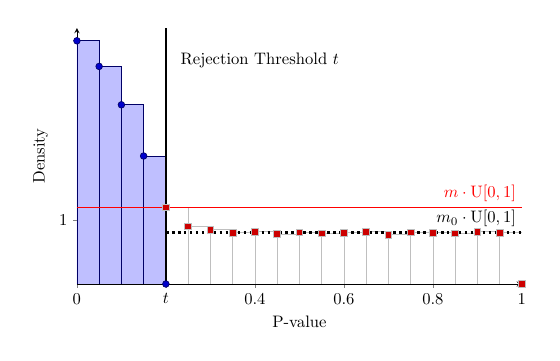
\begin{tikzpicture}[scale=0.6]
\begin{axis}[
    width=11cm,
    height=7cm,
    xlabel={P-value},
    ylabel={Density},
    xmin=0, xmax=1,
    ymin=0, ymax=4,
    xtick={0, 0.2, 0.4, 0.6, 0.8, 1},
    xticklabels={0, $t$, 0.4, 0.6, 0.8, 1},
    ytick={1},
    yticklabels={1},
    axis lines=left,
    enlarge x limits=false,
    legend style={at={(0.5,-0.2)}, anchor=north, legend columns=-1, draw=none}
]

% 1. Denominator R(t): Only shade bars <= t
% Signal Region (0 to t)
\addplot+[
    ybar interval,
    fill=blue!25,
    draw=blue!40!black,
    area legend
] coordinates {
    (0, 3.8) (0.05, 3.4) (0.10, 2.8) (0.15, 2.0) (0.20, 0)
};

% 2. Non-Discoveries: Outlined only
\addplot+[
    ybar interval,
    fill=none,
    draw=gray!50,
    forget plot
] coordinates {
    (0.20, 1.2) (0.25, 0.9) (0.30, 0.85) (0.35, 0.8) 
    (0.40, 0.82) (0.45, 0.78) (0.50, 0.81) (0.55, 0.79) 
    (0.60, 0.8) (0.65, 0.82) (0.70, 0.77) (0.75, 0.81) 
    (0.80, 0.8) (0.85, 0.79) (0.90, 0.82) (0.95, 0.8) (1, 0)
};

% 4. Vertical threshold line
\draw [black, ultra thick] (axis cs:0.20,0) -- (axis cs:0.20,4);
\node at (axis cs:0.22, 3.5) [anchor=west] {Rejection Threshold $t$};

% 5. Horizontal null line (Modified: Solid and Labeled)
\draw [red, thick] (axis cs:0,1.2) -- (axis cs:1,1.2);
\node [red, anchor=south east] at (axis cs:1,1.2) {$m \cdot \textup{U}[0,1]$};

% 6. m0 line (New: Dotted line for p > t)
% Drawn at y=0.8 based on the height of the gray bars
\draw [black, ultra thick, dotted] (axis cs:0.2,0.8) -- (axis cs:1,0.8);
\node [black, anchor=south east] at (axis cs:1,0.8) {$m_0\cdot \textup{U}[0,1]$};

\end{axis}
\end{tikzpicture}
\end{figure}

Choose value $\gamma \in (0,1)$, e.g. 0.5 such that $\hat{\pi}_0 = \frac{\# p_i > \gamma}{m(1-\gamma)}$ and 
\begin{align*}
    (\# p_i > \gamma) \geq \underbrace{(\# \textup{ true nulls } p_i > \gamma )}_{\textup{in expectation: }m_0(1-\gamma)} \overset{\mathbb{E}}{\geq} m_0(1-\gamma).
\end{align*}

\textbf{Adaptive BH}
\begin{itemize}
    \item[1)] Estimate $\pi_0$ with $\hat{\pi}_0$
    \item[2)] Run BH at level $\frac{\alpha}{\hat{\pi}_0}$
\end{itemize}
FDR for BH at level $\frac{\alpha}{\hat{\pi}_0}$ if $\hat{\pi}_0$ is independent of p-values
\begin{align*}
    \textup{FDR} = \mathbb{E}\left[\mathbb{E}[\textup{FDP} \mid \hat{\pi}_0] \right] \leq \alpha \mathbb{E}\left[\frac{\pi_0}{\hat{\pi}_0}\right].
 \end{align*}

\textbf{Problems}
The expectation $\mathbb{E}\left[\frac{\pi_0}{\hat{\pi}_0}\right]$ is infinite if the estimate $\hat{\pi}_0$ is 0 with a non-zero probability. One solution is to add 1 to the numerator of the estimate.

\begin{lemma}
    If $p_i$ are independent, then $\hat{\pi_0}$ with $+1$ correction satisfies $\mathbb{E}\left[\frac{\pi_0}{\hat{\pi}_0}\right] \leq 1$.
\end{lemma}

To achieve independence of the p-values, we should modify BH to account for the fact that $\hat{\pi}_0$ uses the same data. So for a given $\gamma\in[0,1]$, we can use the p-values in $[\gamma,1]$ to estimate $\hat{\pi}_0$, whilst the p-values in $[0,\gamma)$ are candidates for rejection.

\begin{itemize}
    \item[1)] Define $\hat{\pi}_0 := \frac{1+ (\# p_i >\gamma)}{m(1-\gamma)}$
    \item[2)] Find max $k$ such that $p_{(k)} \leq \min\left(\frac{\frac{\alpha}{\hat{\pi}_0}k}{m}, \gamma\right)$  
    \item[3)] Reject $p_{(1)},\dots, p_{(k)}$
\end{itemize}

\begin{thm}{Adaptive BH FDR Bound}{Adabptive BH FDR Bound}
If $p_i$ are independent, then adaptive BH satisfies FDR$\leq \alpha$.
\end{thm}

If $p_i$ are PRDS, adaptive BH may lose FDR control, e.g. $p_1=\dots=p_m\sim\textup{U}[0,1]$, $\gamma=0.5, \alpha \in (0,0.5)$. Then with probability $\frac{1}{2}$ all $p_i > \gamma$ and we make no discoveries, i.e. $\textup{FDP}=0$ and with probability $\frac{1}{2}$, we have $\textup{FDP}=1$.

\textbf{Theory beyond independence}

Asymptotic results: if empiorical distribution of the null $p_i$ converge to $\textup{U}[0,1]$, then FDP converges to a value less than alpha, i.e.
$$\hat{\pi}_0 = \frac{1+ (\# p_i >\gamma)}{m(1-\gamma)} \geq \frac{1+ (\# \textup{ true nulls }p_i >\gamma)}{m(1-\gamma)}\longrightarrow \frac{m_0(1-\gamma)}{m(1-\gamma)} = \pi_0$$

\emph{Note.} FWER/FDR/FDX all only consider binary decisions. We also want to estimate quantitative effect and therefore introduce
\begin{enumerate}
    \item False sign rate (FSR):
    $$\textup{FSR} = \mathbb{E}\left[\frac{\textup{\# discoveries when estimated signs is incorrect}}{\textup{total \# of discoveries}}\right]$$
      \item False coverage rate (FCR):
    $$\textup{FCR} = \mathbb{E}\left[\frac{\textup{\# discoveries for which confidence interval does not contain true parameters}}{\textup{total \# of discoveries}}\right]$$
\end{enumerate}
